\documentclass{beamer}
\setbeamertemplate{caption}[numbered]

\setbeamertemplate{headline}{}
\setbeamertemplate{blocks}{shadow=false}
\setbeamertemplate{footline}{}

\usepackage[citations,footnotes,definitionLists,hashEnumerators,smartEllipses,tightLists=false,hybrid]{markdown}
\usepackage{textpos}
\usepackage{lmodern} % http://ctan.org/pkg/lm
\usepackage{booktabs,multirow}
\usepackage{tcolorbox}

\usepackage{scalerel,stackengine}
\stackMath
\newcommand\reallywidehat[1]{%
\savestack{\tmpbox}{\stretchto{%
  \scaleto{%
    \scalerel*[\widthof{\ensuremath{#1}}]{\kern-.6pt\bigwedge\kern-.6pt}%
    {\rule[-\textheight/2]{1ex}{\textheight}}%WIDTH-LIMITED BIG WEDGE
  }{\textheight}% 
}{0.5ex}}%
\stackon[1pt]{#1}{\tmpbox}%
}
\parskip 1ex

\usetheme{Marburg} %%%% theme
\usefonttheme{structurebold} %%%% choose from: serif, professionalfonts, structurebold, structureitalicserif, structuresmallcapsserif
\usecolortheme{lily}  %%% choose theme color from: albatross, beaver, beetle, crane, default, dolphin, dove, fly, lily, orchid, rose, seagull, seahorse, sidebartab, structure, whale, wolverine

%% \beamertemplatenavigationsymbolsempty                                           
\definecolor{mycolTop}{RGB}{4, 40, 120}
\definecolor{mycolBottom}{RGB}{26, 148, 196}
%\makeatletter
\setbeamertemplate{sidebar canvas right}[vertical shading][top=mycolTop, bottom=mycolBottom]
%\makeatother
\setbeamerfont{section in sidebar}{size=\fontsize{6}{6}\selectfont} %%% set font size and row space
\setbeamerfont{subsection in sidebar}{size=\fontsize{6}{6}\selectfont}
%%\setbeamerfont{section in sidebar shaded}{size=\fontsize{2}{2}\selectfont}


\usepackage{graphicx} % Allows including images
\usepackage{booktabs} % Allows the use of \toprule, \midrule and \bottomrule in tables
\usepackage{subcaption}
\usepackage{amsmath,amsfonts,amsthm,bm} 
\usepackage[square,sort,comma]{natbib}

%\usepackage{natbib} 
%\bibliographystyle{apalike}

\usepackage{listings,lstautogobble}
\usepackage{xcolor}
\definecolor{RoyalBlue}{cmyk}{1, 0.50, 0, 0}
\lstset{language=R,
	keywordstyle=\color{RoyalBlue},
	basicstyle=\normalsize\ttfamily,
	commentstyle=\ttfamily\itshape\color{gray},
	stringstyle=\ttfamily,
	showstringspaces=false,
	breaklines=true,
	frameround=ffff,
	frame=single,
	rulecolor=\color{black},
	autogobble=true
}


\newcommand{\iid}{\textrm{i.i.d.\ }}
\newcommand{\E}{\mathrm{E}}
\newcommand{\Var}{\mathrm{Var}}
\newcommand{\Cov}{\mathrm{Cov}}
\newcommand{\Corr}{\mathrm{Corr}}
\newcommand{\tr}{\mathrm{tr}}
\newcommand\inv[1]{#1\raisebox{1.15ex}{$\scriptscriptstyle-\!1$}}


%----------------------------------------------------------------------------------------
%	TITLE PAGE
%----------------------------------------------------------------------------------------

\title[]{Data Visualisation Using \texttt{R}} 

\subtitle{\textcolor{magenta}{Lecture-4}}

\author[]{Suman Rakshit} % Your name
\institute[School of EECMS, Curtin University] % Your institution as it will appear on the bottom of every slide, may be shorthand to save space
{
	\textcolor{magenta}{School of EECMS, Curtin University} % Your institution for the title page
	%\medskip
	%\textit{abc@abc.com} % Your email address
}
%\date{14 September, 2020, SAGI Symposium} % Date, can be changed to a custom date

\titlegraphic{
\includegraphics[width=0.4\textwidth,
height=0.18\textheight]{PlotsLec4/CURTIN}}

\begin{document}



\begin{frame}
	\titlepage % Print the title page as the first slide
\end{frame}


\addtobeamertemplate{frametitle}{}{%
	\begin{textblock*}{100mm}(0\textwidth,8cm)
		
\includegraphics[height=0.8cm,width=2cm]{PlotsLec4/CURTIN}
\end{textblock*}}




%----------------------------------------------------------------------------------------
%	PRESENTATION SLIDES
%----------------------------------------------------------------------------------------

%------------------------------------------------ 
\section{Outline}
\begin{frame}[t]\frametitle{Outline}
\begin{enumerate}
\item Dates: different convention of representing
\item Correct way to represent Dates
\item Dates in \texttt{R}
\item Datetime object in \texttt{R}
\item Datetime handling in \texttt{lubridate}
\item Creating time-series plots
\item Visualisation of spatial data
\end{enumerate}
\end{frame}


%\setbeamercovered{transparent}

\section{Different conventions}
\begin{frame}\frametitle{How do we represent Date in \textcolor{red}{\textsf{R}}?}
If you write \textcolor{red}{11th February of 2021} as $$11-02-2021$$ in \textsf{R},
you will get
\begin{figure}
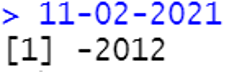
\includegraphics[width=0.50\linewidth]{PlotsLec4/DateAsNumber}
\end{figure}
\end{frame}

\begin{frame}\frametitle{How do we represent Date in \textcolor{red}{\textsf{R}}?}
If you put quotes around $11-02-2021$, it may work: $$``11-02-2021"$$

But check the class of this object:
\begin{figure}
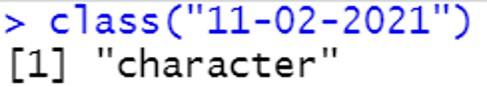
\includegraphics[width=0.70\linewidth]{PlotsLec4/DateAsChar}
\end{figure}
\end{frame}

\setbeamercovered{transparent}
\begin{frame}\frametitle{Different convention of representing dates}
\begin{itemize}
\item Added confusion arises due to different conventions of representing the same date.
\vspace{0.3in}
\item<2-> In Australia, the date \textcolor{red}{11th February of 2021} may be represented either by $11-02-2021$ or by $11/02/2021$, or by $11/2/21$, or simply `11th Feb, 2021'. We like to follow the \textcolor{red}{Day-Month-Year} format.
\vspace{0.3in}
\item<3-> In USA, on the other hand, the same date may be written as $02-11-2021$, or as $2/11/2021$ or $2/11/21$, or `Feb 11, 2021'. In USA they follow the \textcolor{red}{Month-Day-Year} format.
\end{itemize}
\end{frame}


\begin{frame}{How to represent 11th Feb 2021}
\begin{figure}

\includegraphics[width=0.50\linewidth]{PlotsLec4/WhichFormatCorrect}
\end{figure}
\end{frame}

\section{Correct way to represent Dates}
\begin{frame}\frametitle{Global standard -- ISO 8601}
It turns out that there is a global standard of presenting dates (introduced in 1988), called ISO 8601 standard.
\begin{figure}

\includegraphics[width=0.99\linewidth]{PlotsLec4/ISO}
\end{figure}
\end{frame}

\setbeamercovered{transparent}
\begin{frame}\frametitle{ISO 8601 Date properties}
\begin{itemize}
\item ISO 8601 states that the three components of a date should be written in the \textcolor{blue}{decreasing order of time} units, i.e., first the \textcolor{red}{year}, then the \textcolor{red}{month}, and finally, the \textcolor{red}{day}.
\vspace{0.15in}

\item<2-> Each time component should have a \textcolor{blue}{fixed number of digits} -- \textcolor{red}{Year} should be \textcolor{red}{4 digits}, \textcolor{red}{Month} should be \textcolor{red}{2 digits}, and \textcolor{red}{Day} should be \textcolor{red}{2 digits}.
\vspace{0.15in}

\item<3-> Because of the last point, the \textcolor{blue}{single digit} days and months \textcolor{blue}{should be padded with a leading zero}.
\vspace{0.15in}

\item<4-> You do not need a \textcolor{red}{separator}, but if you use a \textcolor{red}{separator}, it has to be a \textcolor{red}{dash}. So, the \textcolor{red}{11th Feb of 2021} will be written in ISO 8601 as $$2021-02-11$$.
\end{itemize}
\end{frame}

\section{Dates in \texttt{R}}

\begin{frame}\frametitle{Use \textcolor{red}{\texttt{as.Date()}} to create a Date object}
\begin{figure}
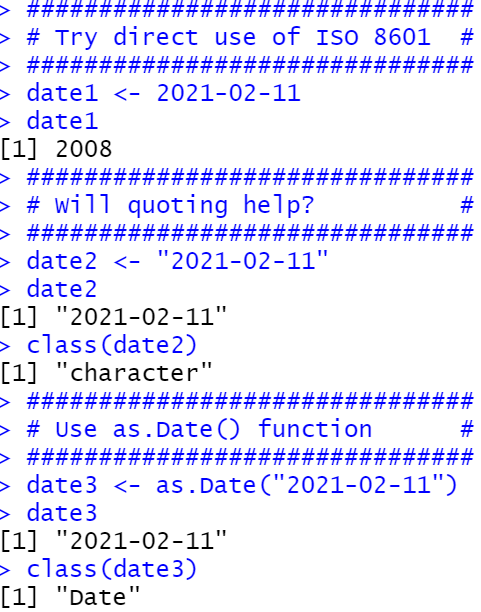
\includegraphics[width=0.60\linewidth]{PlotsLec4/AsDate}
\end{figure}
\end{frame}

\begin{frame}\frametitle{Quiz: which one is correct ISO8601 format?}
\textcolor{red}{\texttt{as.Date()}} will \textcolor{blue}{only accept ISO-8601} formatted dates. 

So, which one is the correct ISO 8601 date format for \textcolor{red}{16th August of 2021}?
{\Large

\begin{enumerate}
\centering
\item "16-8-2021"
\item "2021-16-08"
\item "2021-08-16"
\item "2021-8-16"
\end{enumerate} 
}
\end{frame}

\setbeamercovered{transparent}
\begin{frame}\frametitle{Mathematical operations with Dates}
\begin{itemize}
\item Behind the scenes, Dates are stored as number of days since 1970-01-01.
\vspace{0.15in}
\item<2-> As a result, we can perform standard mathematical comparisons and computations.
\vspace{0.15in}
\item<3-> We can ask if one date comes after another date: \textcolor{blue}{\texttt{as.Date("2021-08-16")}$>$\texttt{as.Date("2021-08-01")}}\\ The answer will be \texttt{\textcolor{red}{TRUE}}.
\vspace{0.15in}
\item<4-> We can add days:
\textcolor{blue}{\texttt{as.Date("2021-08-16")}$+$ 1} gives the answer \textcolor{red}{\texttt{"2021-08-17"}}.
\vspace{0.10in}
\item<5-> We can find the difference between dates:\\
\textcolor{blue}{\texttt{as.Date("2022-08-16")}} $ - $ \textcolor{blue}{\texttt{as.Date("2021-08-16")}} gives the answer \texttt{\textcolor{red}{365 days}}.
\end{itemize}
\end{frame}

\begin{frame}[fragile]{RCode: Plotting with Date objects}
\begin{lstlisting}
# Create three Dates
Date <- c(as.Date("2021-06-01"), 
          as.Date("2021-07-01"), 
          as.Date("2021-08-01"))
# Create a time-series
Price <- c(50, 200, 100)
# Create the time-series dataset
data <- data.frame(Date, Price)
# Plot the time-series
ggplot(data, aes(Date, Price)) + 
  geom_line() + geom_point() + 
  theme_classic()
\end{lstlisting}
\end{frame}

\begin{frame}\frametitle{Plot of the time-series}
\begin{figure}
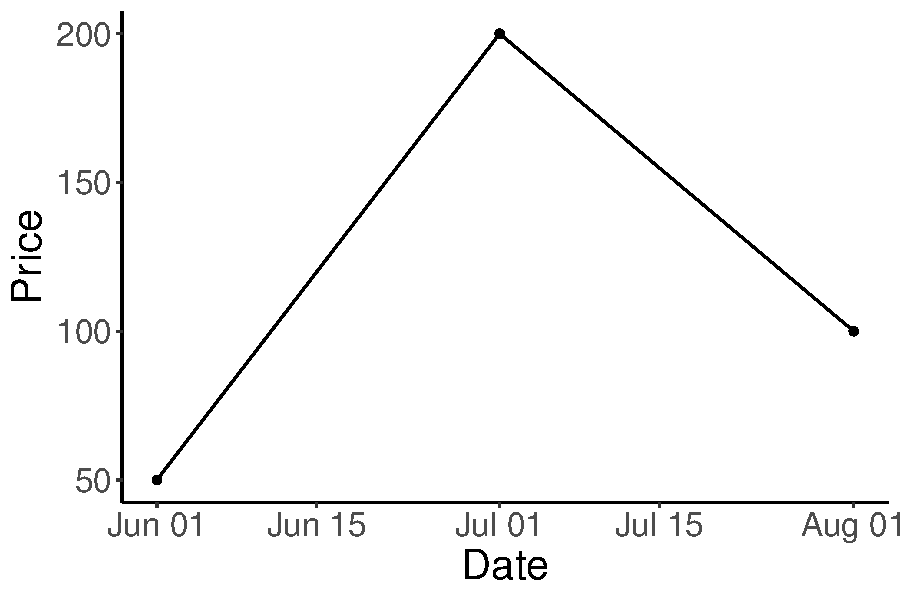
\includegraphics[width=0.99\linewidth]{PlotsLec4/TimeSeries}
\end{figure}
\end{frame}

\begin{frame}\frametitle{Plot of real-life time-series}
\begin{figure}
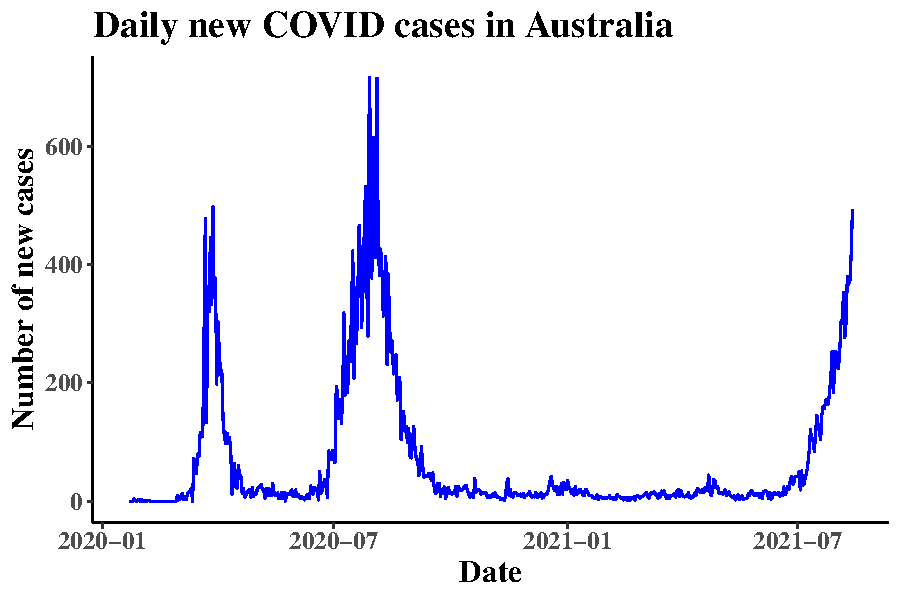
\includegraphics[width=0.99\linewidth]{PlotsLec4/CovidSeries}
\end{figure}
\end{frame}

\section{Datetime object in \texttt{R}}

\begin{frame}\frametitle{Let's talk about \textbf{\textcolor{red}{Time}}}
\begin{enumerate}
\item ISO 8601 convention is to put time units again in the decreasing order: \textcolor{blue}{\textbf{HH:MM:SS}}. 
\vspace{0.3in}
\item Each time unit should have fixed number of digits:
\begin{itemize}
\item Hours: 00--24
\item Minutes: 00--59
\item Seconds: 00--60 (60 only for leap seconds)
\end{itemize}
\vspace{0.3in}
\item Can use no or \texttt{:} as separator.
\end{enumerate}
\end{frame}

\begin{frame}\frametitle{\textbf{\textcolor{red}{Datetimes}} objects in \texttt{\textcolor{red}{R}}}
\begin{itemize}
\item Datetimes can be stored using two objects
\begin{enumerate}
\item \texttt{POSIXlt} -- list with named components
\item \texttt{POSIXct} -- seconds since 1970-01-01 00:00:00
\end{enumerate} 
\item \texttt{POSIXct} is better suited to be stored in a Data Frame column.
\item \texttt{as.POSIXct()} turns a ISO 8601 datetime string into a \texttt{POSIXct object}.
\end{itemize}
\end{frame}

\begin{frame}\frametitle{Quiz: which one is valid ISO 8601 format?}
Which one is the valid ISO-8601 Datetime representation for 6:30 pm of 11th February of 2021.
{\Large

\begin{enumerate}
\centering
\item "2021-02-11 06:30:00"
\item "2021-02-11 06:00:30"
\item "2021-02-11 18:00:30"
\item "2021-02-11 18:30:00"
\end{enumerate} 
}
\end{frame}

\begin{frame}[fragile]\frametitle{Example of using \texttt{as.POSIXct()}}
\begin{lstlisting}
# Define 6:30 pm of 11th Feb, 2021 as a string
dtmString <- "2021-02-11 18:30:00"
# Create the Datetime object
dtm <- as.POSIXct(dtmString)
\end{lstlisting}
\begin{figure}
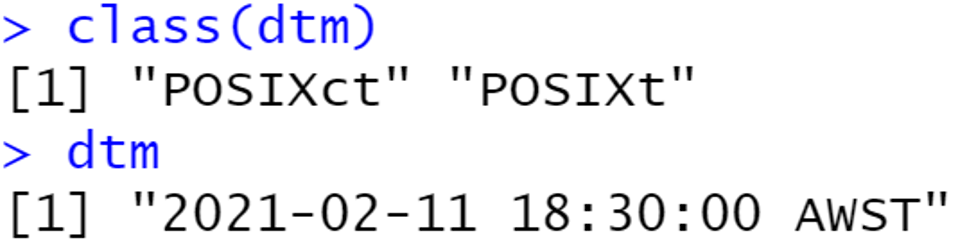
\includegraphics[width=0.99\linewidth]{PlotsLec4/DatetimeObj}
\end{figure}
\end{frame}

\setbeamercovered{transparent}

\begin{frame}\frametitle{Let's talk about \textbf{\textcolor{red}{Timezones}}}
\begin{itemize}
\item In ISO 8601 convention, if no timezone is specified, the local timezone is assumed: 
\begin{itemize}
\item "2021-02-11T18:30:00" -- 6:30 pm Local Time on 11th Feb, 2021
\end{itemize}
\vspace{0.3in}
\item<2-> If you add a "Z" at the end of Datetime specification, then a UTC timezone is assumed:
\begin{itemize}
\item "2021-02-11T18:30:00Z" -- 6:30 pm UTC (coordinated universal time) on 11th Feb, 2021
\end{itemize}
\vspace{0.3in}
\item<3-> In ISO 8601 convention, any other timezone is defined as the offset from the UTC timezone:
\begin{itemize}
\item "2021-02-11T18:30:00+08:00" -- 6:30 pm in Perth
\end{itemize}
\end{itemize}
\end{frame}

\begin{frame}\frametitle{Timezone specification in \texttt{\textcolor{red}{as.POSIXct()}}}
Unfortunately, \texttt{\textcolor{red}{as.POSIXct}} does not recognise ISO-8601 timezone specifications.
\begin{figure}
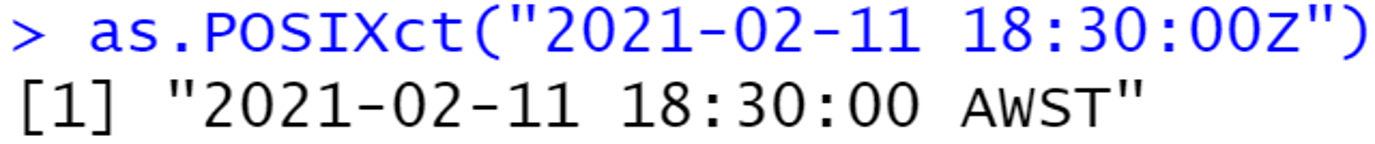
\includegraphics[width=0.60\linewidth]{PlotsLec4/Posixct}
\caption{{\scriptsize UTC specification shows local timezone -- AWST stands for Australian Western Standard Time (UTC+8)}.}
\end{figure}
To specify a time zone, you have to access the \textcolor{red}{\texttt{tz}} parameter in the function \textcolor{red}{\texttt{as.POSIXct}}:
\begin{figure}
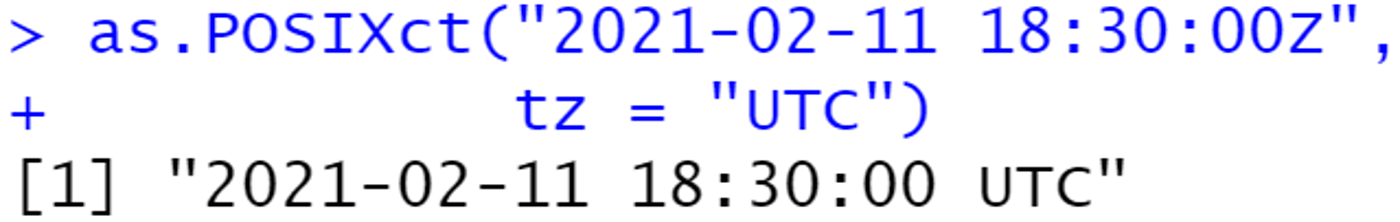
\includegraphics[width=0.60\linewidth]{PlotsLec4/PosixctWithTz}
\caption{{\scriptsize \textcolor{red}{\texttt{tz = "UTC}}} sets the UTC timezone.}
\end{figure}
\end{frame}


\begin{frame}\frametitle{Operations with \texttt{\textcolor{red}{Datetime}} objects}
\begin{figure}
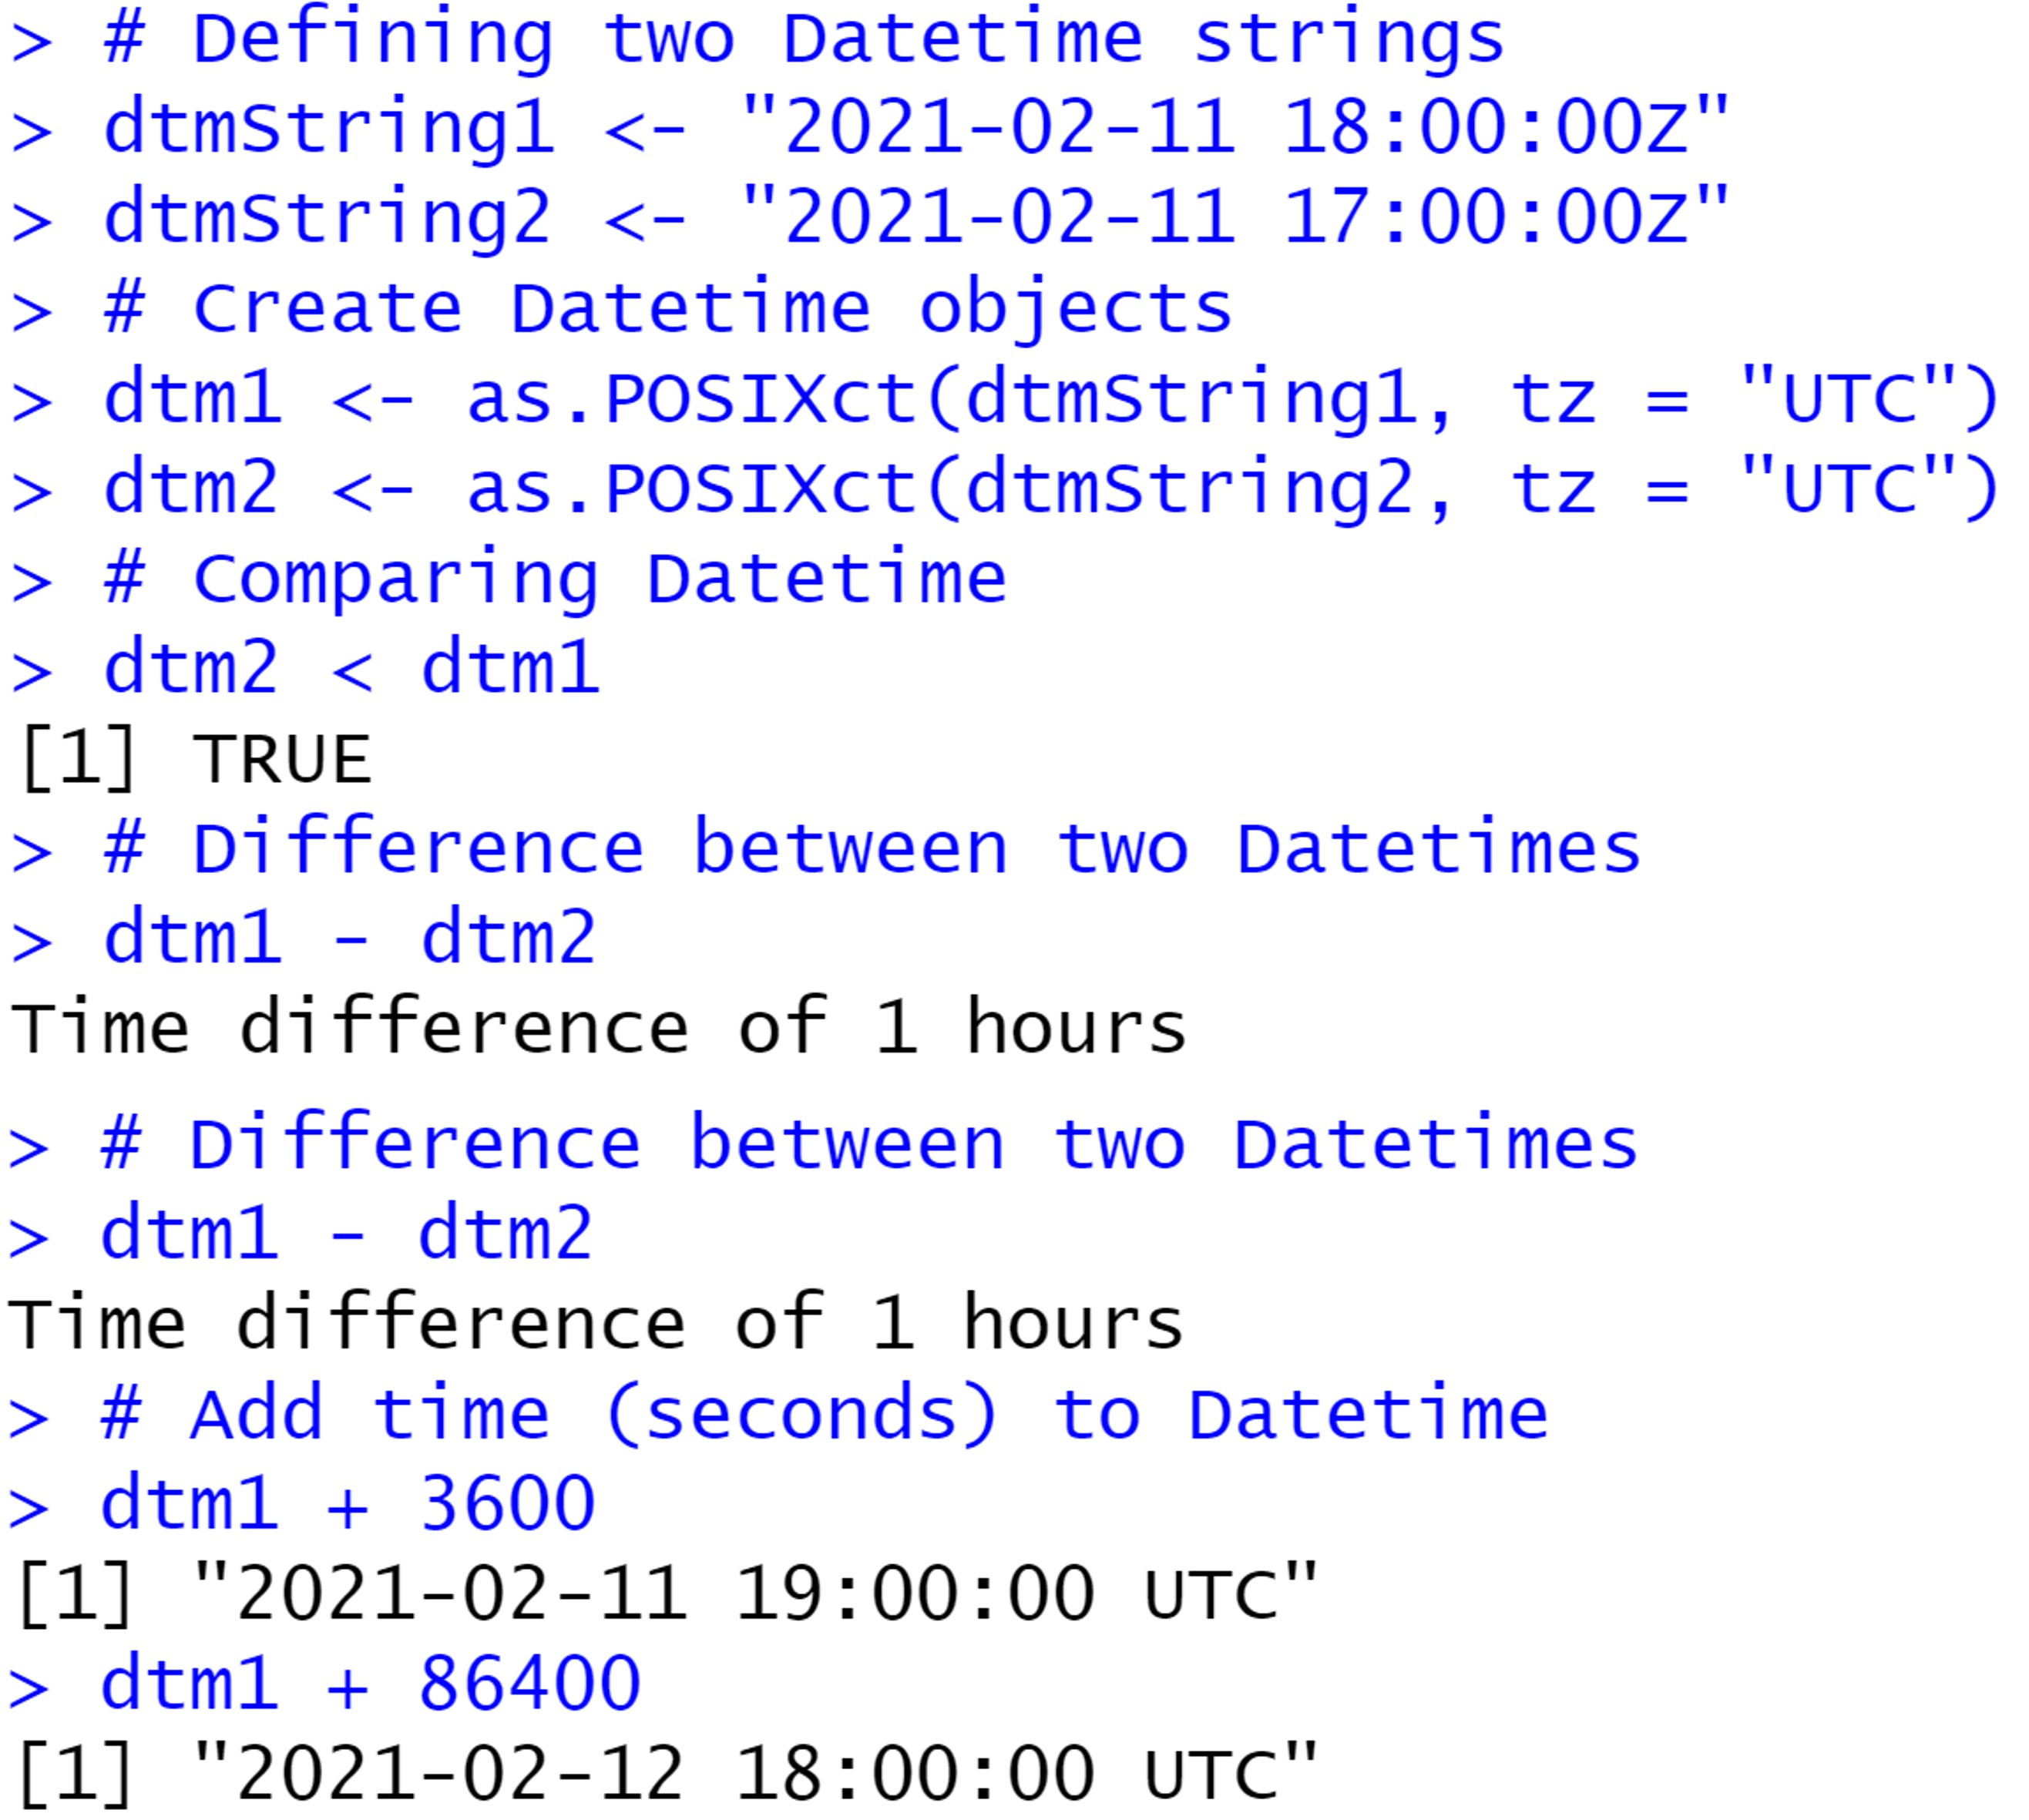
\includegraphics[width=0.85\linewidth]{PlotsLec4/DatetimeOperations}
\end{figure}
\end{frame}

\begin{frame}[fragile]\frametitle{RCode: plotting datetime objects}
\begin{lstlisting}
# Create three consecutive hours
Time <- c(as.POSIXct("2021-02-11 18:00:00"),
 as.POSIXct("2021-02-11 19:00:00"),
 as.POSIXct("2021-02-11 20:00:00"))
# Create price data
Price <- c(100, 250, 320)
# Create hourly timeseries
data <- data.frame(Time, Price)
# Plot hourly timeseries
ggplot(data, aes(Time, Price)) +
   geom_line() +  geom_point() +
   theme_classic() +
ggtitle("Example of an hourly timeseries")
\end{lstlisting}
\end{frame}

\begin{frame}\frametitle{Plot of hourly data}
\begin{figure}
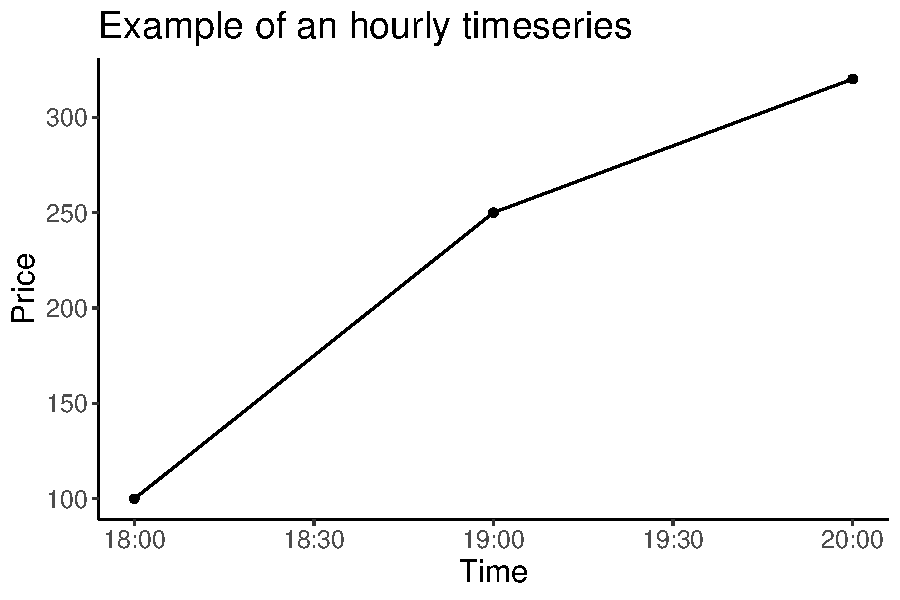
\includegraphics[width=0.99\linewidth]{PlotsLec4/HourlySeries}
\end{figure}
\end{frame}

\section{Datetime handling in \texttt{lubridate}}

\setbeamercovered{transparent}
\begin{frame}\frametitle{\texttt{\textcolor{red}{lubridate}} makes handling Datetime easy}
\begin{itemize}
\item \texttt{\textcolor{red}{lubridate}} makes it as easy as possible to work with \textcolor{red}{date and time} in \texttt{\textcolor{red}{R}}.

\vspace{0.2in}
\item <2-> \texttt{\textcolor{red}{lubridate}} is part of the \texttt{\textcolor{red}{tidyverse}} -- which means
\begin{itemize}
\item it works well with built-in datetime objects;
\item it works well with other tidyverse packages;
\item function names are very intuitive and easy to work with.
\end{itemize}

\vspace{0.2in}

\item<3-> \texttt{\textcolor{red}{lubridate}} allows consistent behaviour regardless of the underlying datetime object;

\vspace{0.2in}
\item<4-> You just need to learn one \texttt{\textcolor{red}{lubridate}} function to achieve a given task for any \texttt{\textcolor{red}{datetime}} object -- be it stored in a \texttt{\textcolor{red}{Date}} object, or in a \texttt{\textcolor{red}{POSIXct}} object, or in any other timeseries objects such as \texttt{\textcolor{red}{xts}} or \texttt{\textcolor{red}{zoo}}.
\end{itemize}
\end{frame}

\begin{frame}\frametitle{Key Date functions in \texttt{\textcolor{red}{lubridate}}}
\begin{figure}
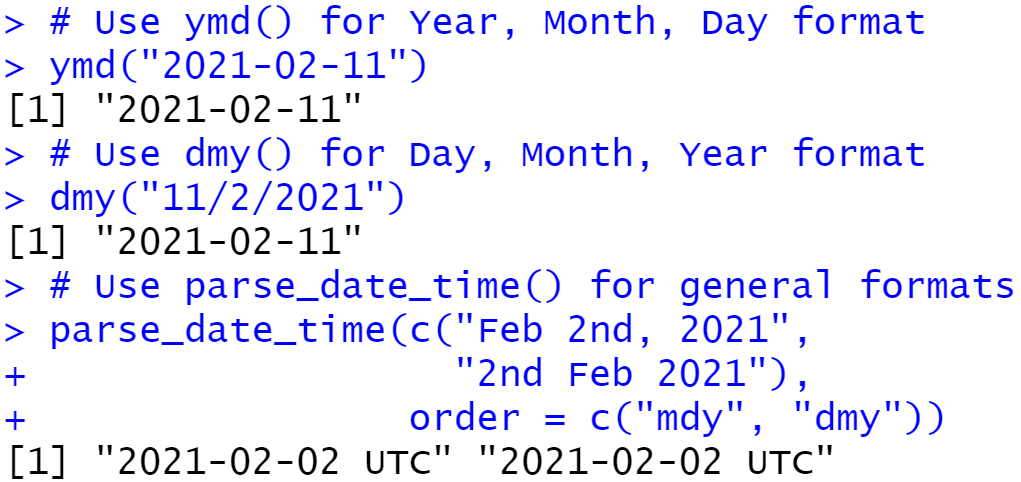
\includegraphics[width=0.99\linewidth]{PlotsLec4/LubDateFns}
\caption{{\small \texttt{\textcolor{red}{ymd()}}, \texttt{\textcolor{red}{mdy()}}, and \texttt{\textcolor{red}{parse$\_$date$\_$time()}} are versatile functions for converting almost any legal Date specification into the universally accepted ISO 8601 format.}}
\end{figure}
\end{frame}


\begin{frame}[fragile]{RCode: key Date functions in \texttt{\textcolor{red}{lubridate}}}
\begin{lstlisting}
# Use ymd() for Year, Month, Day format
ymd("2021-02-11")
# Use dmy() for Day, Month, Year format
dmy("11/2/2021")
# Use parse_date_time() for general formats
parse_date_time(c("Feb 2nd, 2021",
                  "2nd Feb 2021"),
                order = c("mdy", "dmy"))
\end{lstlisting}
\end{frame}

\begin{frame}\frametitle{\texttt{\textcolor{red}{lubridate}} functions for extracting features}
\begin{figure}
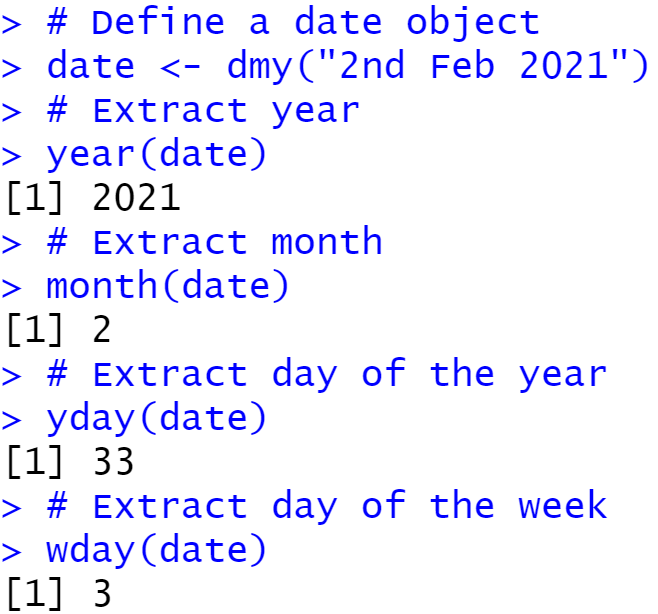
\includegraphics[width=0.70\linewidth]{PlotsLec4/DateFeatures}
\caption{{\small \texttt{\textcolor{red}{year()}}, \texttt{\textcolor{red}{month()}}, \texttt{\textcolor{red}{yday()}}, and \texttt{\textcolor{red}{wday()}} are great functions to extract useful date related features.}}
\end{figure}
\end{frame}

\begin{frame}\frametitle{Example: Covid-19 data summary}
\begin{figure}
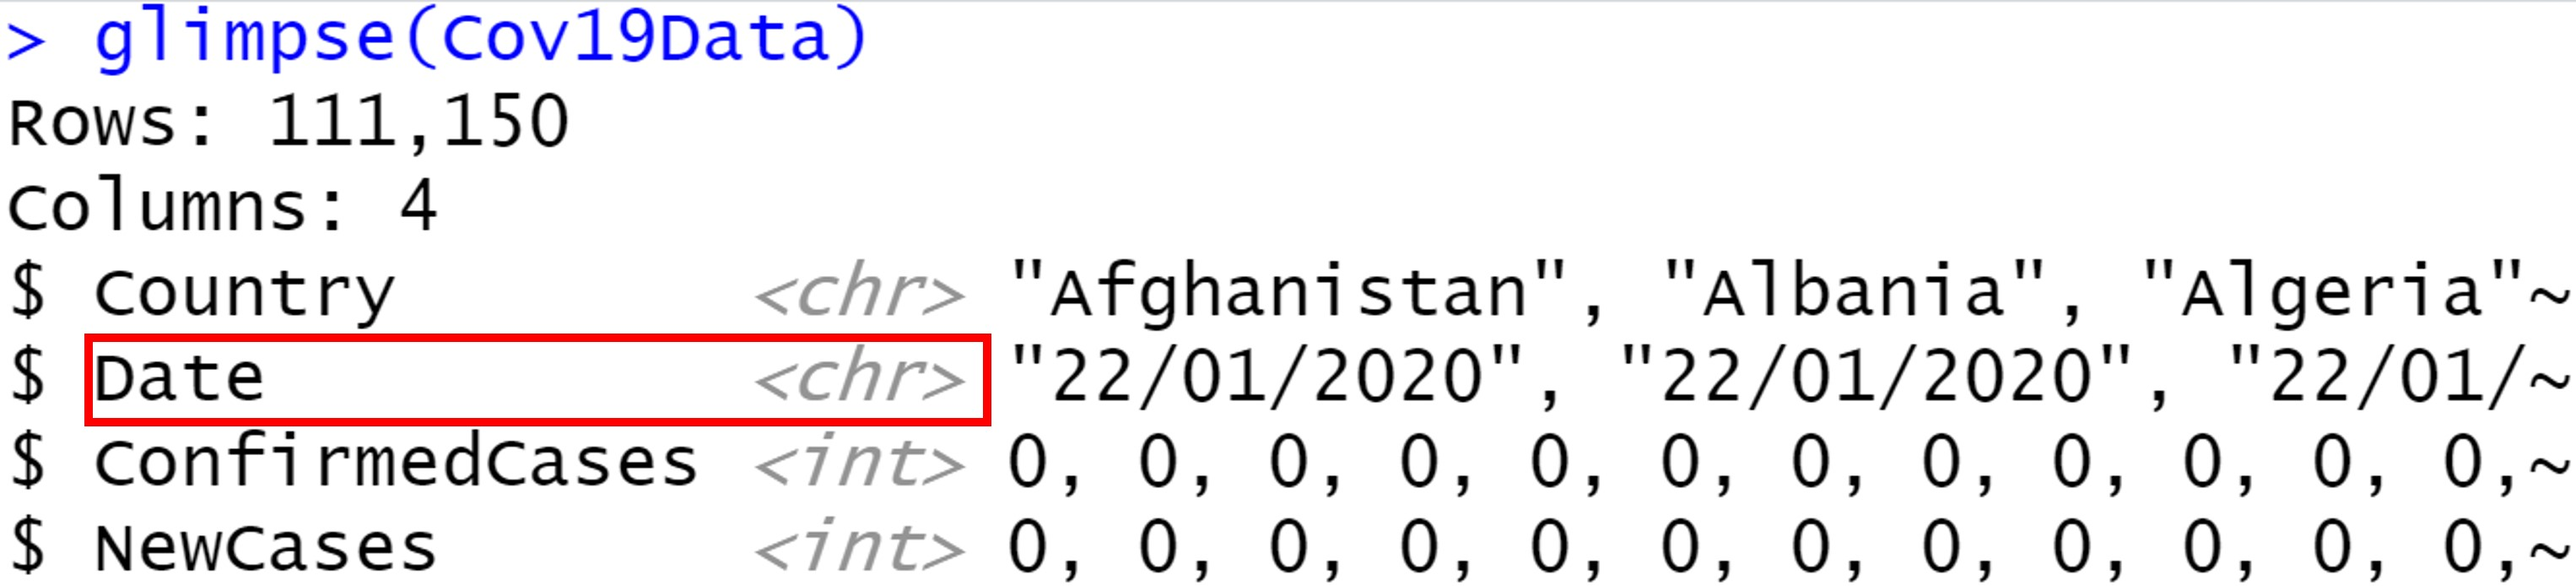
\includegraphics[width=0.99\linewidth]{PlotsLec4/Cov19DataSummary}
\end{figure}
We can turn the \textcolor{red}{Date} variable into a vector of \texttt{\textcolor{red}{Date}} elements using the \texttt{\textcolor{red}{dmy()}} function.
\begin{figure}
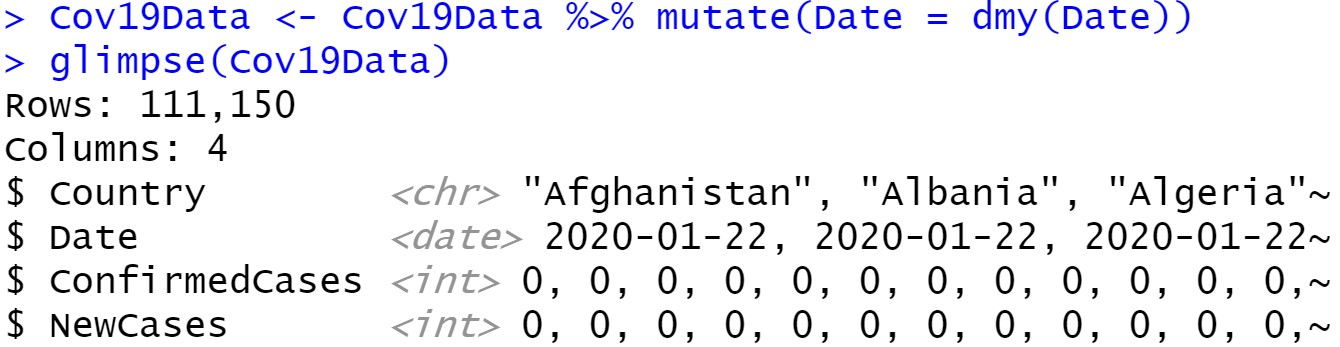
\includegraphics[width=0.99\linewidth]{PlotsLec4/Cov19DataSummary2}
\end{figure}
\end{frame}

\section{Creating time-series plots}
\begin{frame}\frametitle{Timeseries plot using \texttt{\textcolor{red}{geom$\_$line()}}}
\begin{figure}
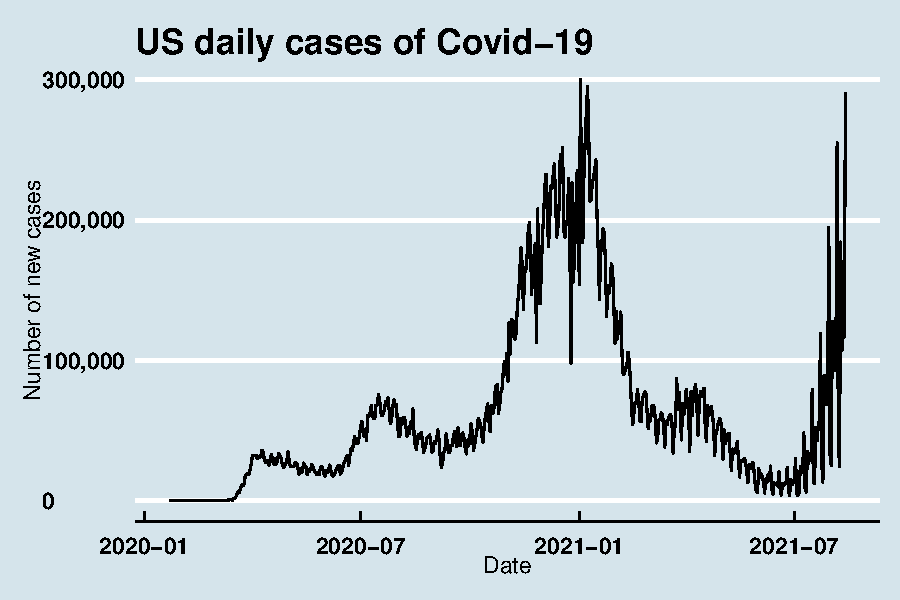
\includegraphics[width=0.99\linewidth]{PlotsLec4/covidUSA_baseplt}
\end{figure}
\end{frame}

\begin{frame}[fragile]\frametitle{RCode: timeseries plot using \texttt{\textcolor{red}{geom$\_$line()}}}
\begin{lstlisting}
# Filter USA data
Cov19USA <- Cov19Data %>% 
            filter(Country == "US")
# Timeseries plot of Covid cases
ggplot(Cov19USA , aes(Date, NewCases)) +
 geom_line() + 
 theme_economist() +
 scale_y_continuous(labels = scales::comma) +
 theme(axis.text = element_text(face="bold")) +
 labs(y = "Number of new cases")+
 ggtitle("US daily cases of Covid-19")
\end{lstlisting}
\end{frame}

\begin{frame}\frametitle{Better labelling of Dates}
\begin{figure}
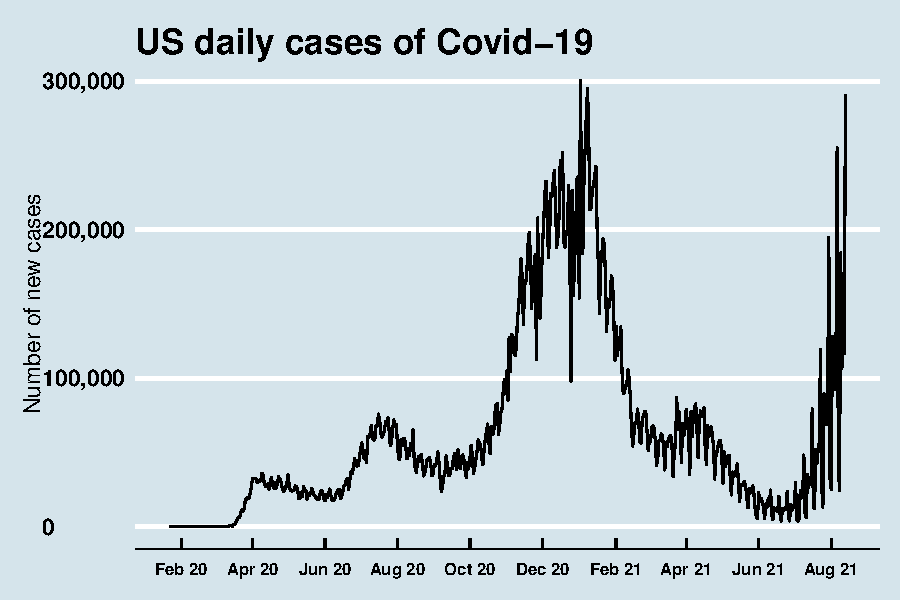
\includegraphics[width=0.99\linewidth]{PlotsLec4/Covid19_US_2}
\end{figure}
\end{frame}

\begin{frame}[fragile]\frametitle{RCode: better labeling via \texttt{\textcolor{red}{scale$\_$x$\_$date()}}}
\begin{lstlisting}
covidUSA_baseplt +
# Show Month and Year with 2 month breaks
scale_x_date(date_breaks = "2 month",
             date_labels = "%b %y") 
\end{lstlisting}
\end{frame}

\begin{frame}\frametitle{List of Date labels}
\begin{figure}
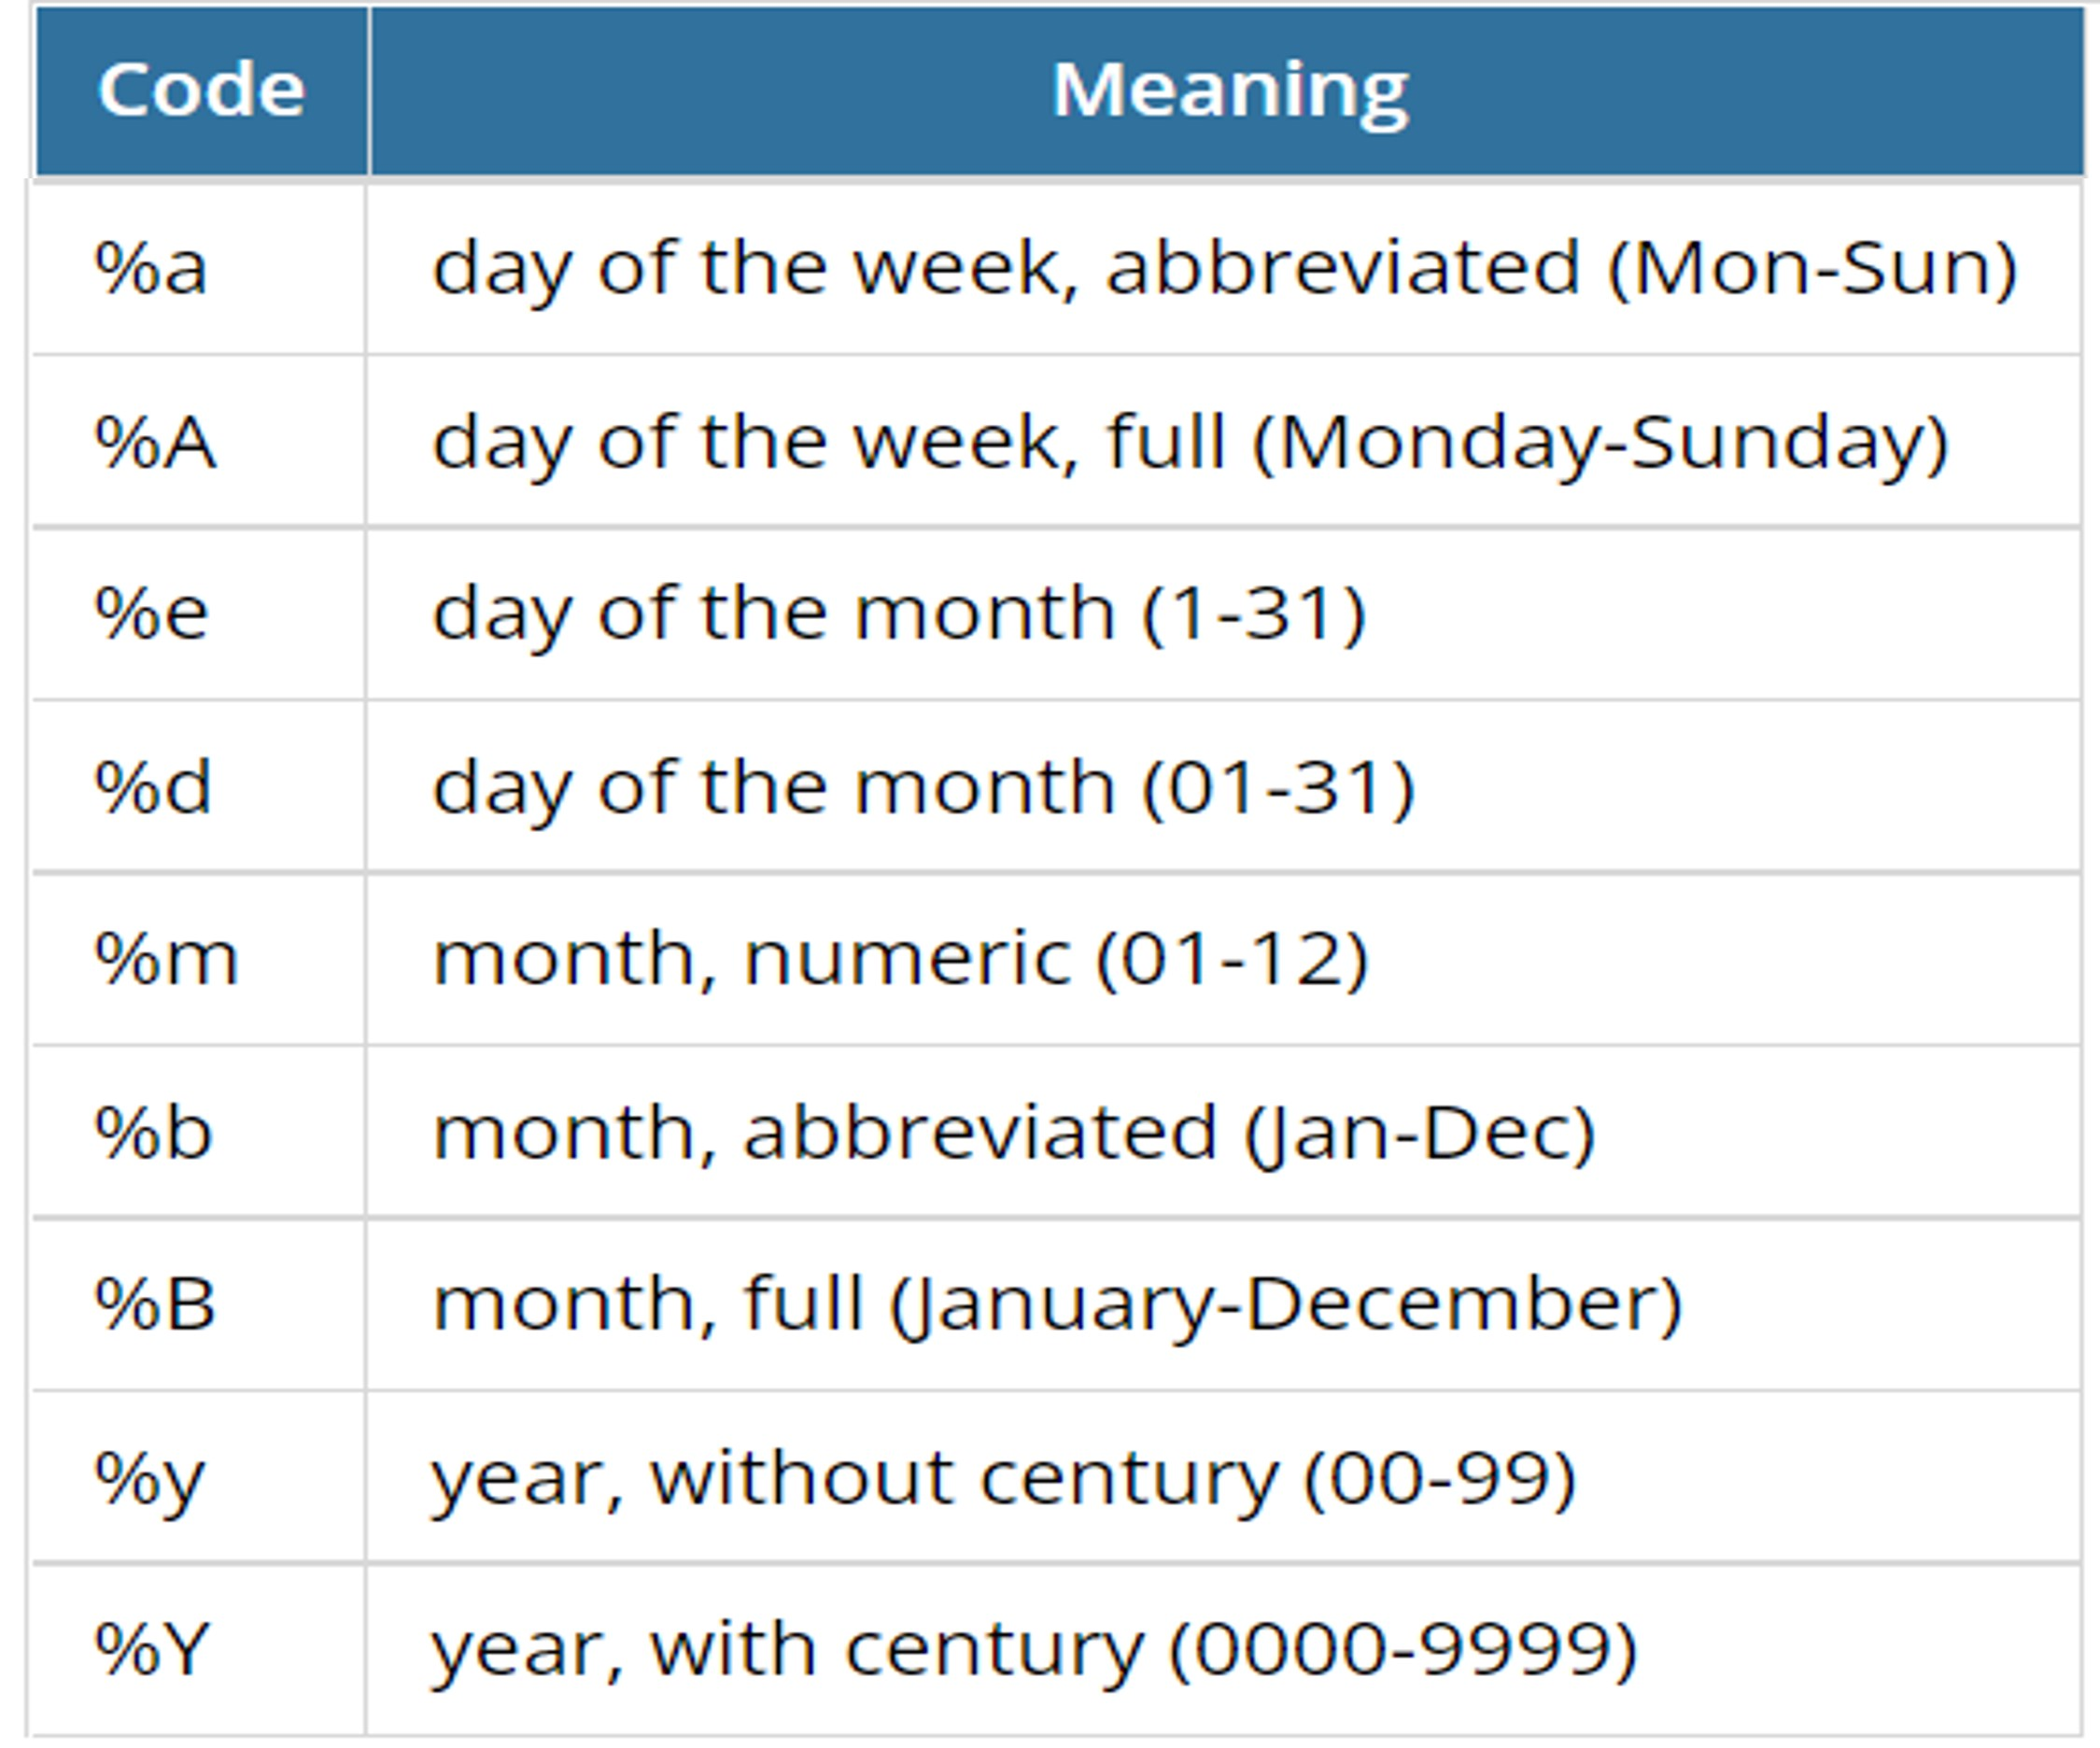
\includegraphics[width=0.80\linewidth]{PlotsLec4/DateLabels}
\caption{{\small For \texttt{\textcolor{red}{date$\_$labels}} argument in \texttt{\textcolor{red}{scale$\_\star \_$date()}}}}
\end{figure}
\end{frame}

\begin{frame}\frametitle{Another labelling example of dates}
\begin{figure}
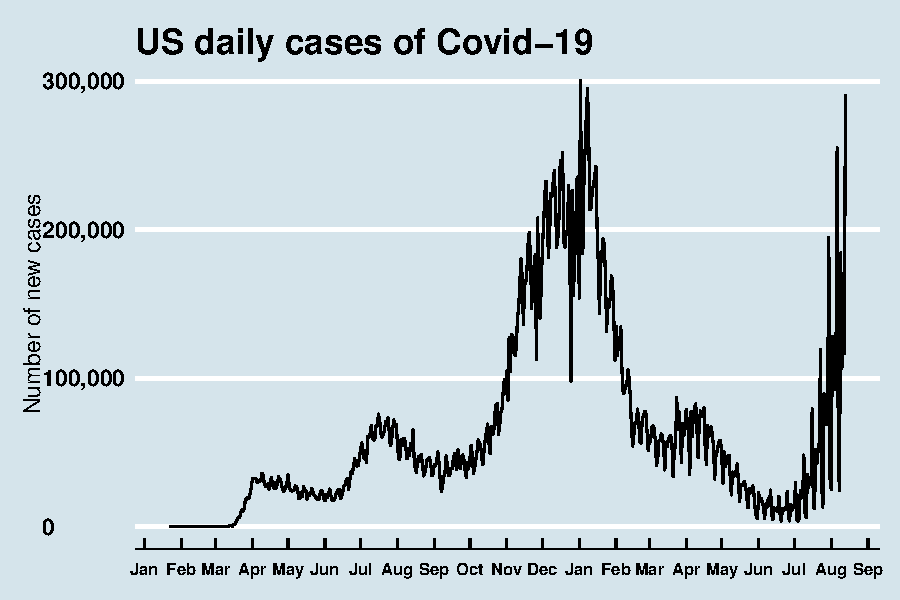
\includegraphics[width=0.99\linewidth]{PlotsLec4/Covid19_US_3}
\caption{\small{We have introduced monthly labels on the date axis.}}
\end{figure}
\end{frame}

\begin{frame}[fragile]\frametitle{RCode: month label using \texttt{\textcolor{red}{scale$\_$x$\_$date()}}}
\begin{lstlisting}
covidUSA_baseplt +
# Show Month labels for each month
scale_x_date(date_breaks = "1 month",
             date_labels = "%b") 
\end{lstlisting}
\end{frame}

\begin{frame}\frametitle{Comparing US and Australia Covid-19 data}
\begin{figure}
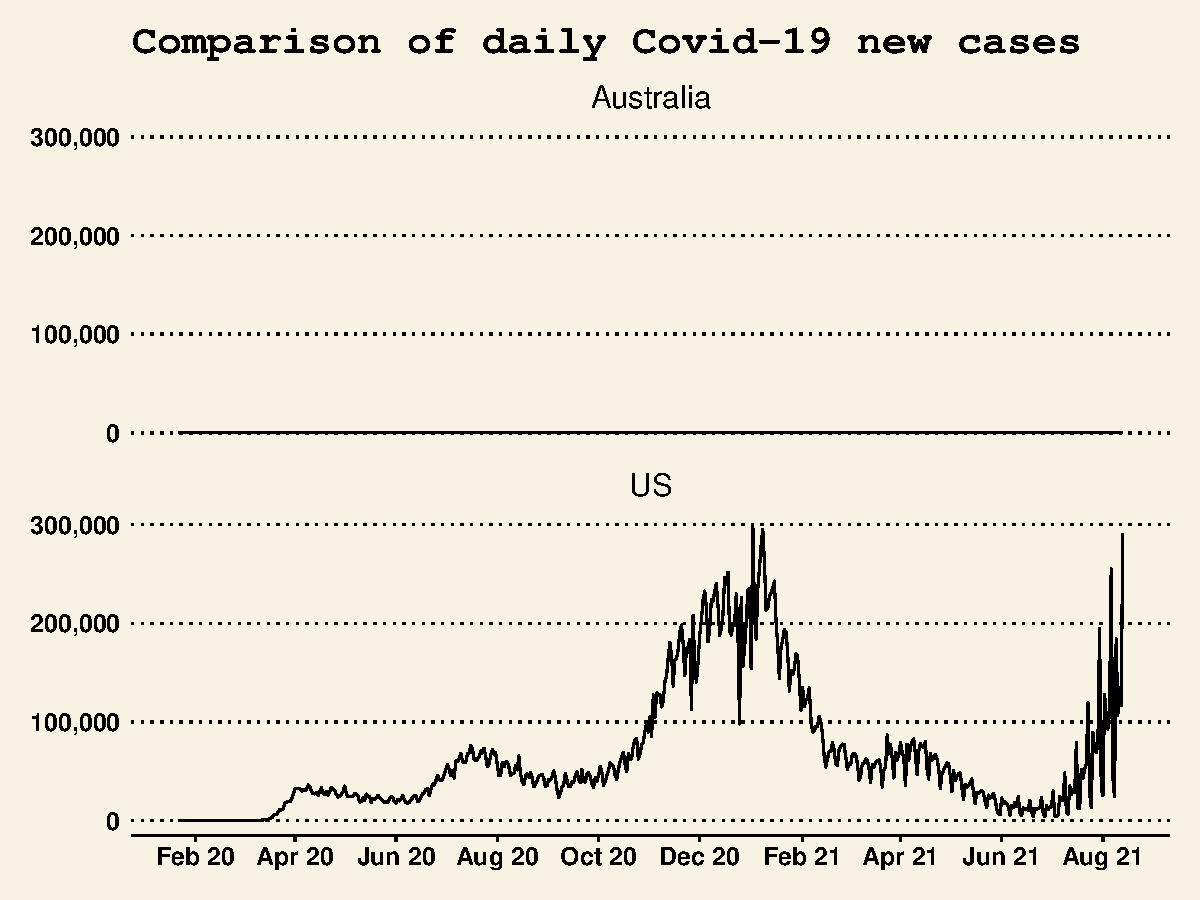
\includegraphics[width=0.99\linewidth]{PlotsLec4/Cov19USA_Ausplt}
\end{figure}
\end{frame}

\begin{frame}\frametitle{Use \texttt{\textcolor{red}{scales = "free$\_$y"}} in \texttt{\textcolor{red}{facet$\_$wrap()}}}
\begin{figure}
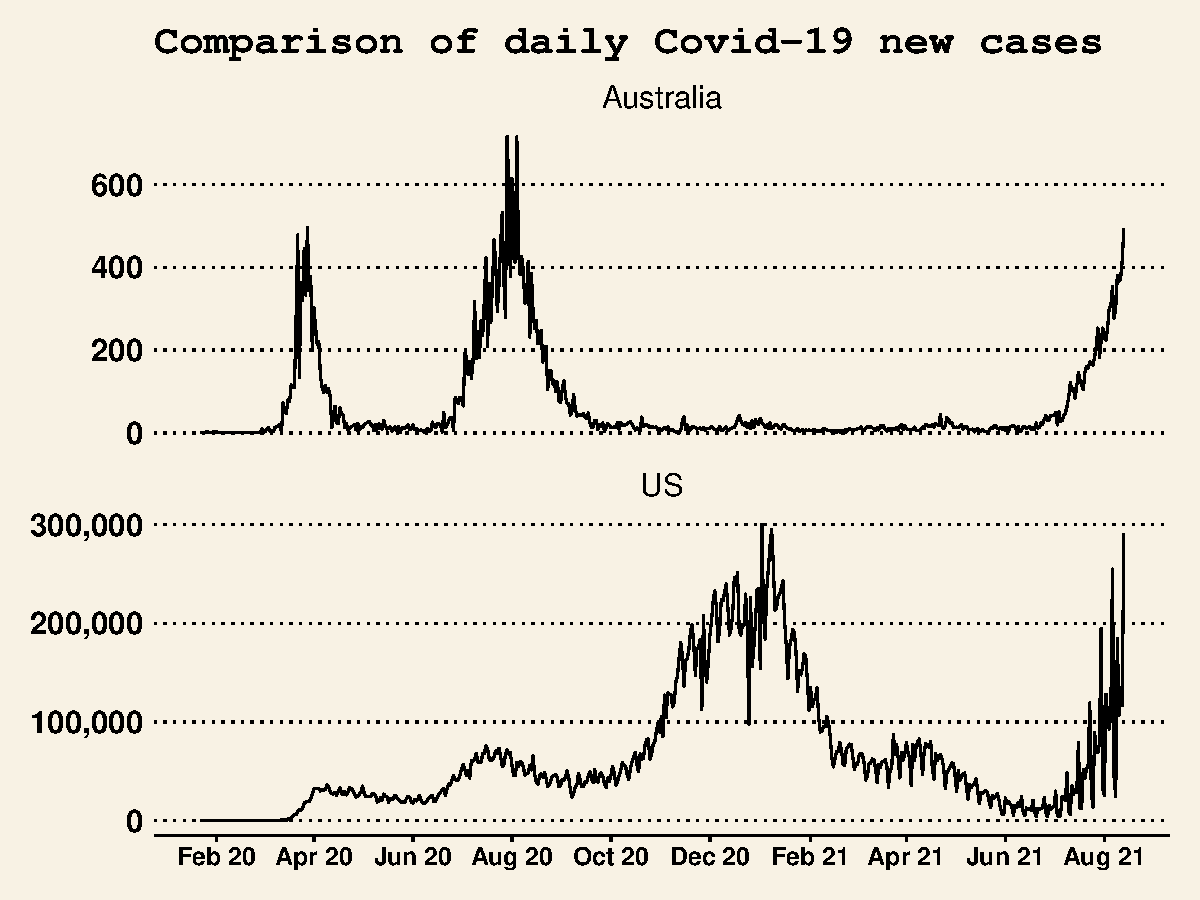
\includegraphics[width=0.99\linewidth]{PlotsLec4/Cov19USA_Ausplt2}
\end{figure}
\end{frame}

\begin{frame}[fragile]\frametitle{RCode:\texttt{\textcolor{red}{scales = "free$\_$y"}} in \texttt{\textcolor{red}{facet$\_$wrap()}}}
\begin{lstlisting}
#####################################
# Default facet_wrap() uses common  #
# scale for both x and y variables  #
#####################################
facet_wrap(~ Country, 
             nrow = 2) 
\end{lstlisting}

\begin{lstlisting}
#####################################
# Use different scales for USA and  #
# Australian daily Covid cases      #
#####################################   
facet_wrap(~ Country, 
             nrow = 2,
             scales = "free_y") 
\end{lstlisting}
\end{frame}

\begin{frame}\frametitle{Use \texttt{\textcolor{red}{geom$\_$area()}} for advanced plotting}
\begin{figure}
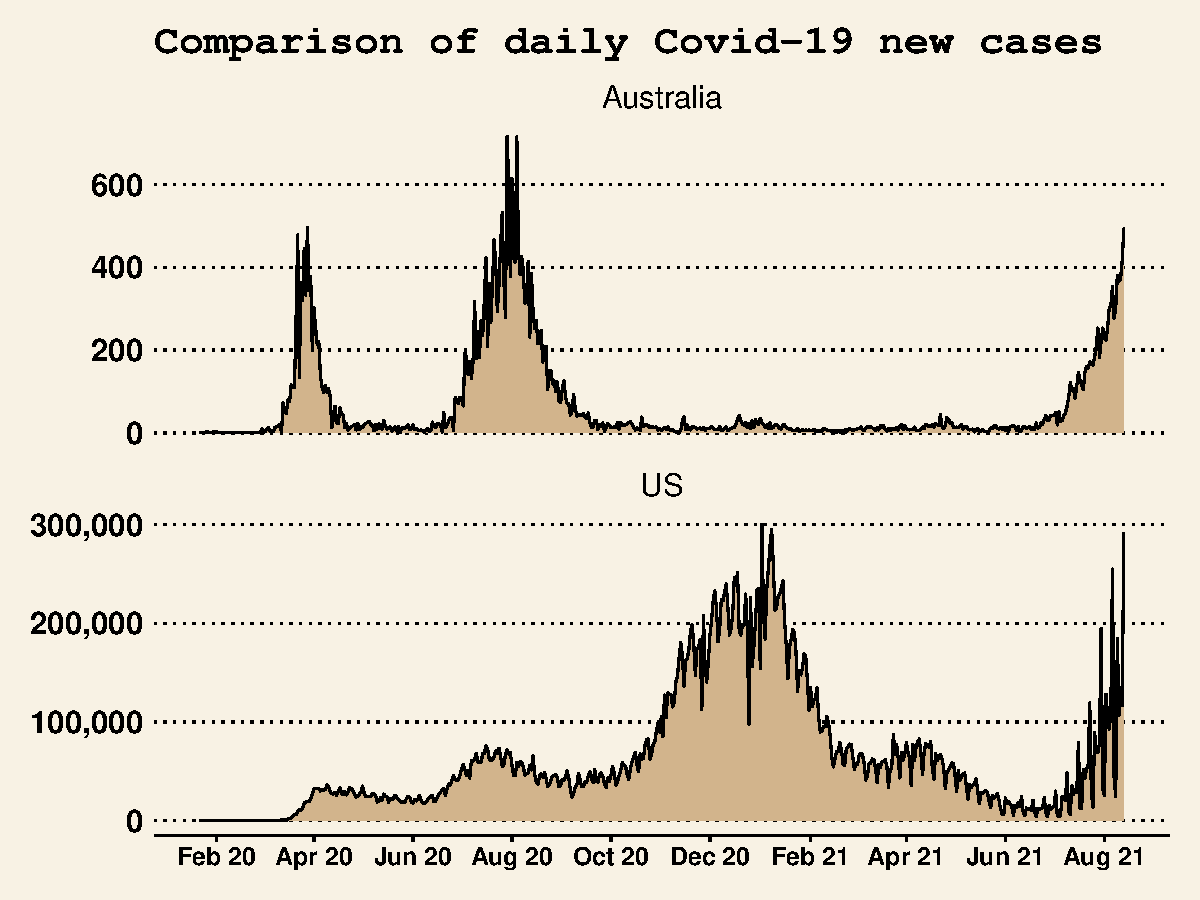
\includegraphics[width=0.99\linewidth]{PlotsLec4/Cov19USA_AusAreaplt}
\end{figure}
\end{frame}


\section{Visualisation of spatial data}

\begin{frame}
\centering 
{\Large \textcolor{blue}{Visualisation of Spatial Data}}
\end{frame}

\setbeamercovered{transparent}
\begin{frame}\frametitle{Making maps in R}
\begin{itemize}
\item To draw a map, we need mainly two things:
\begin{enumerate}
\item The map -- polygons constituting a geographical region. For example, the world map with polygons given for each country or the map of USA with polygons given for 51 states in the USA. 
\item The variable -- colors or mark to fill in the polygons based on the variable values.
\end{enumerate}
\item<2->Typically for a real-life spatial data problem, you should have the shapefile corresponding to your map. Then, the variable values may come in a separate file, and you may have to merge the map and the variables so that you have a proper mapping of variables onto polygons constituting the map/study region.
\item<3-> Once you map variables onto the polygons, you can create colorful maps known as Choropleths.
\end{itemize}
\end{frame}

\begin{frame}\frametitle{Plotting the World map}
\begin{figure}
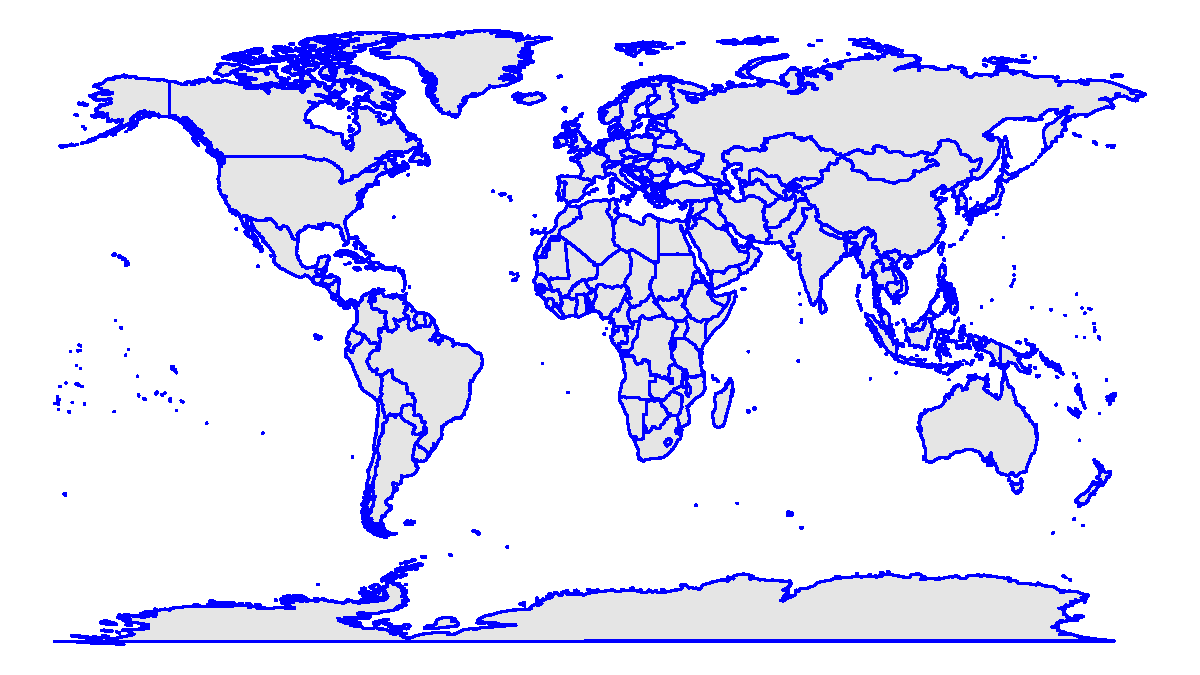
\includegraphics[width=0.99\linewidth]{PlotsLec4/WorldMap}
\end{figure}
\end{frame}

\begin{frame}[fragile]\frametitle{RCode: plotting the World map}
\begin{lstlisting}
library(maps)
# Read in the World map
WorldMap <- map_data("world")
# Plot WorldMap using geom_polygon()
ggplot(WorldMap, aes(long, lat)) +
  geom_polygon(aes(group = group),
               fill="gray90",
               color = "blue") +
  theme_void() 
\end{lstlisting}
\end{frame}

\begin{frame}\frametitle{Plotting filtered data -- India and China}
\begin{figure}
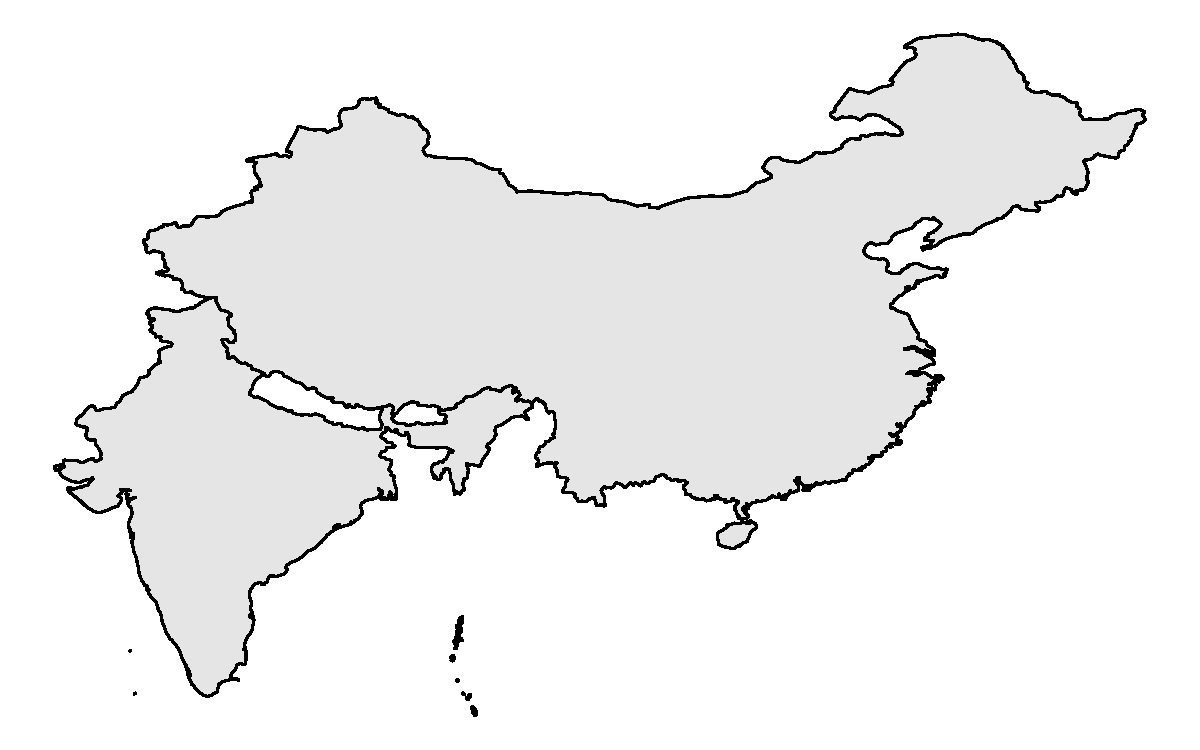
\includegraphics[width=0.99\linewidth]{PlotsLec4/IndoChinaMap}
\end{figure}
\end{frame}

\begin{frame}[fragile]\frametitle{RCode: plotting a subset of the World map}
\begin{lstlisting}
# Get the map for India and China
indoChina <- WorldMap %>% 
  filter(region %in% c("India",
                        "China"))

# Plot Indo-China region using geom_polygon()
ggplot(indoChina, aes(long, lat)) +
  geom_polygon(aes(group = group),
               fill = "gray90",
               color = "black") +
  theme_void() 
\end{lstlisting}
\end{frame}

\begin{frame}\frametitle{Map of USA states}
\begin{figure}
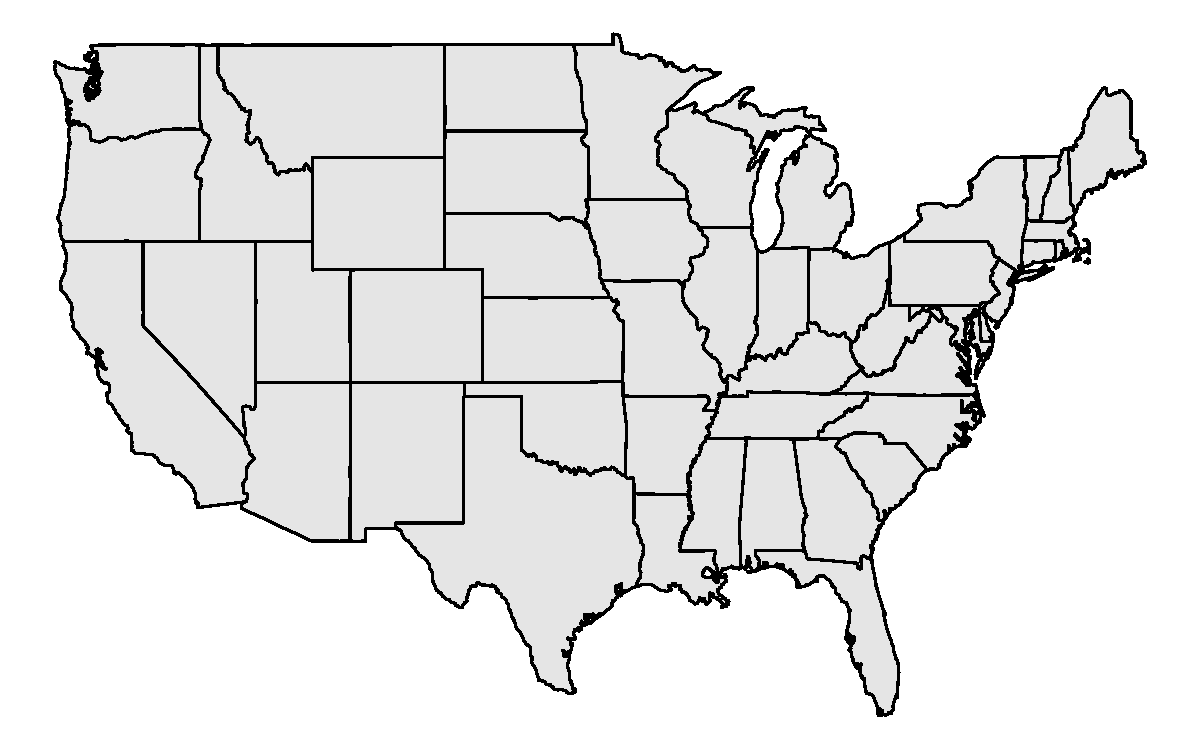
\includegraphics[width=0.99\linewidth]{PlotsLec4/UsaMap}
\end{figure}
\end{frame}

\begin{frame}[fragile]\frametitle{RCode: plotting the map of USA states}
\begin{lstlisting}
library(maps)
# Read in the USA map
usaMap <- map_data("state")
# Plot the USA map using geom_polygon()
ggplot(usaMap, aes(long, lat)) +
  geom_polygon(aes(group = group),
               fill="gray90",
               color = "black") +
  theme_void() 
\end{lstlisting}
\end{frame}

\begin{frame}[fragile]\frametitle{RCode: create data to fill in map polygons}
\begin{lstlisting}
# Get all USA states
states <- unique(usaMap$region)
# Create fake data for all states
set.seed(123)
qualVar <- sample(LETTERS[1:5], 49, 
                  replace=TRUE)
set.seed(3011)
quantVar <- runif(49, 0, 25)
# Create the data frame
dataForUSMap <- data.frame(
         region = states,
         QualVar = qualVar,
         QuantVar = quantVar)
\end{lstlisting}
\end{frame}

\begin{frame}[fragile]\frametitle{RCode: merge variable data with USA map}
\begin{lstlisting}
#####################################
# Merge the data frame dataForUSMap #
# with the USA state map data       #
#####################################
usaMapMerged <- usaMap %>%
                left_join(dataForUSMap,
                          by = "region")
########################################
# Choropleth using Qualitative variable#
########################################                          
ggplot(usaMapMerged, aes(long, lat,
                    group = group,
                    fill = QualVar)) +
  geom_polygon(color = "black") +
  theme_void()
\end{lstlisting}
\end{frame}

\begin{frame}\frametitle{US map: choropleth using qualitative data}
\begin{figure}
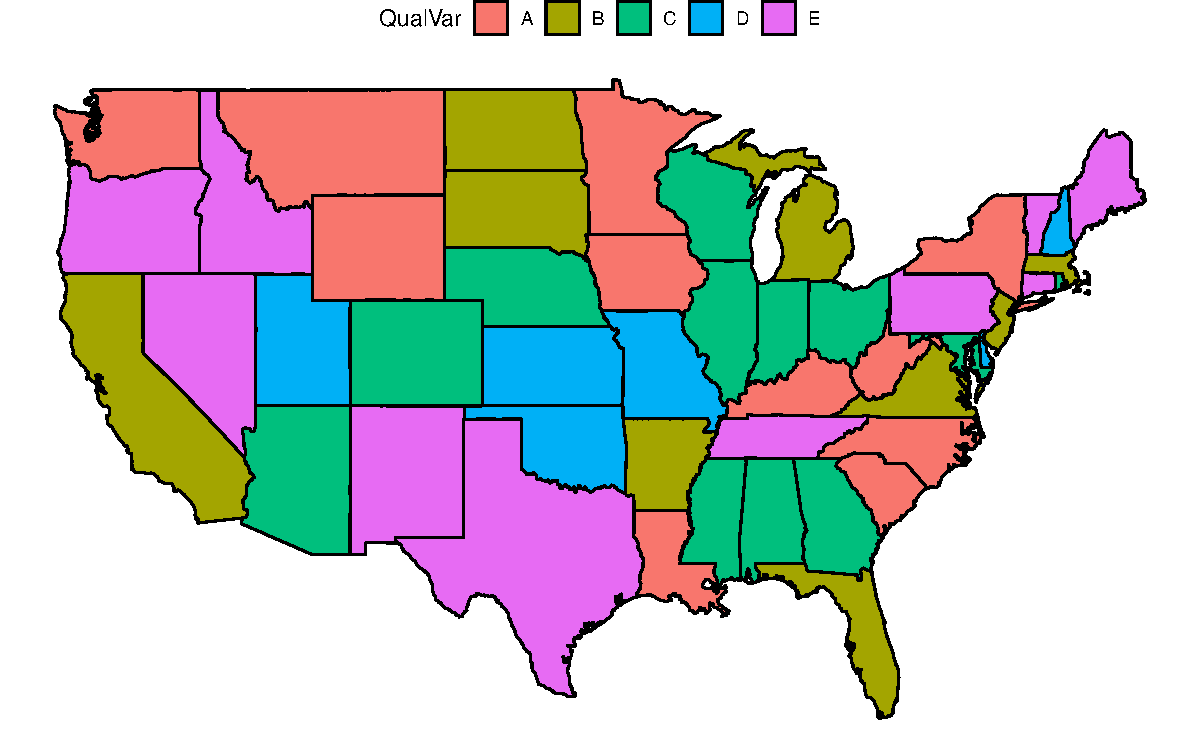
\includegraphics[width=0.99\linewidth]{PlotsLec4/UsaChoroplethQual}
\end{figure}
\end{frame}

\begin{frame}\frametitle{Choropleth with Spectral color palette}
\begin{figure}
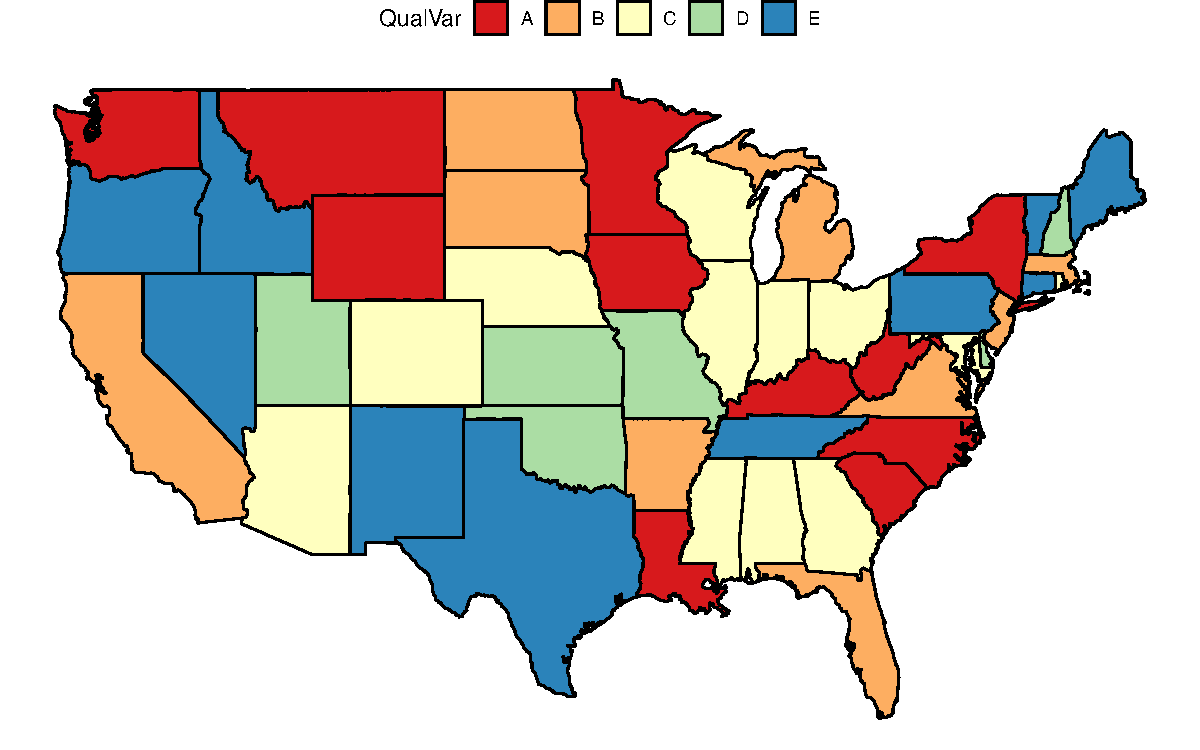
\includegraphics[width=0.99\linewidth]{PlotsLec4/UsaChoroplethQual2}
\caption{{\small Added \texttt{\textcolor{red}{scale$\_$fill$\_$brewer(palette = "Spectral")}} with the last plot.}}
\end{figure}
\end{frame}

\begin{frame}[fragile]\frametitle{Choropleth using quantitative variable}
\begin{lstlisting}
########################################
#Choropleth using Quantitative variable#
########################################                          
ggplot(usaMapMerged, aes(long, lat,
                    group = group,
                    fill = QuantVar)) +
  geom_polygon(color = "black") +
  theme_void()
\end{lstlisting}
\end{frame}

\begin{frame}\frametitle{US map: choropleth using quantitative data}
\begin{figure}
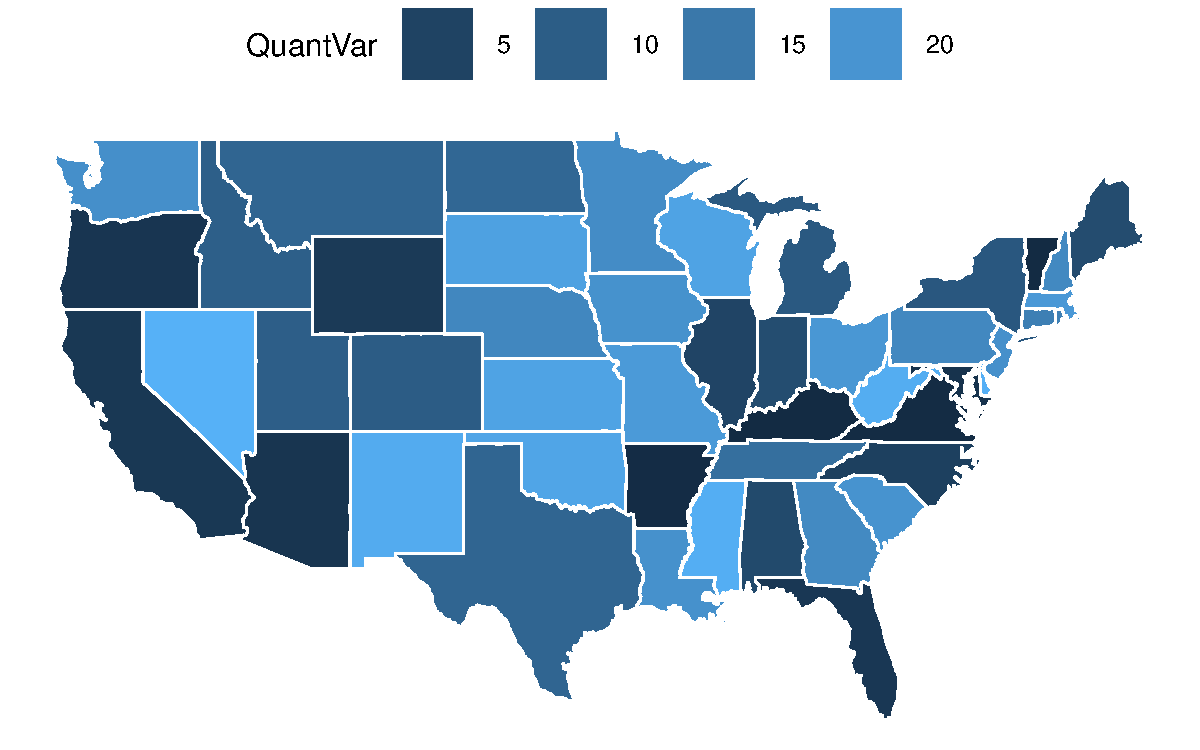
\includegraphics[width=0.99\linewidth]{PlotsLec4/UsaChoroplethQuant}
\end{figure}
\end{frame}

\begin{frame}\frametitle{Improved color by \texttt{\textcolor{red}{scale$\_$fill$\_$gradientn()}}}
\begin{figure}
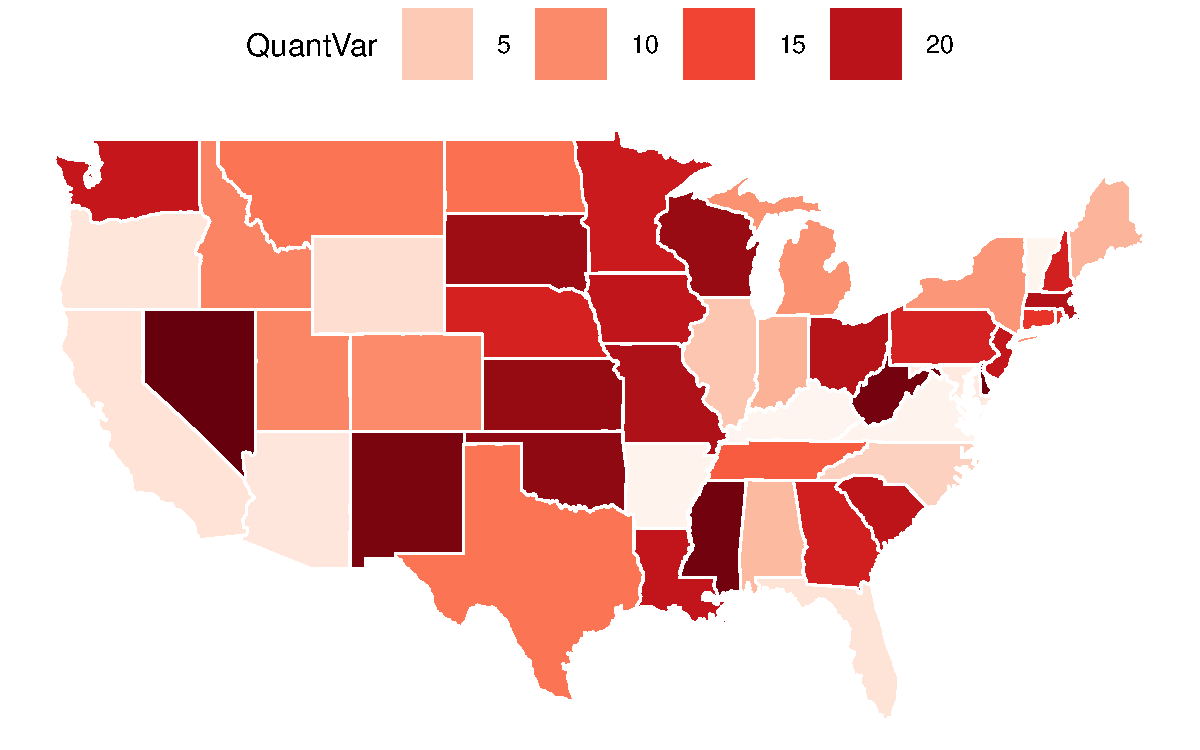
\includegraphics[width=0.99\linewidth]{PlotsLec4/UsaChoroplethQuant2}
\end{figure}
\end{frame}

\begin{frame}\frametitle{Real-life data example: \textcolor{red}{\texttt{murders}} data}
\begin{figure}
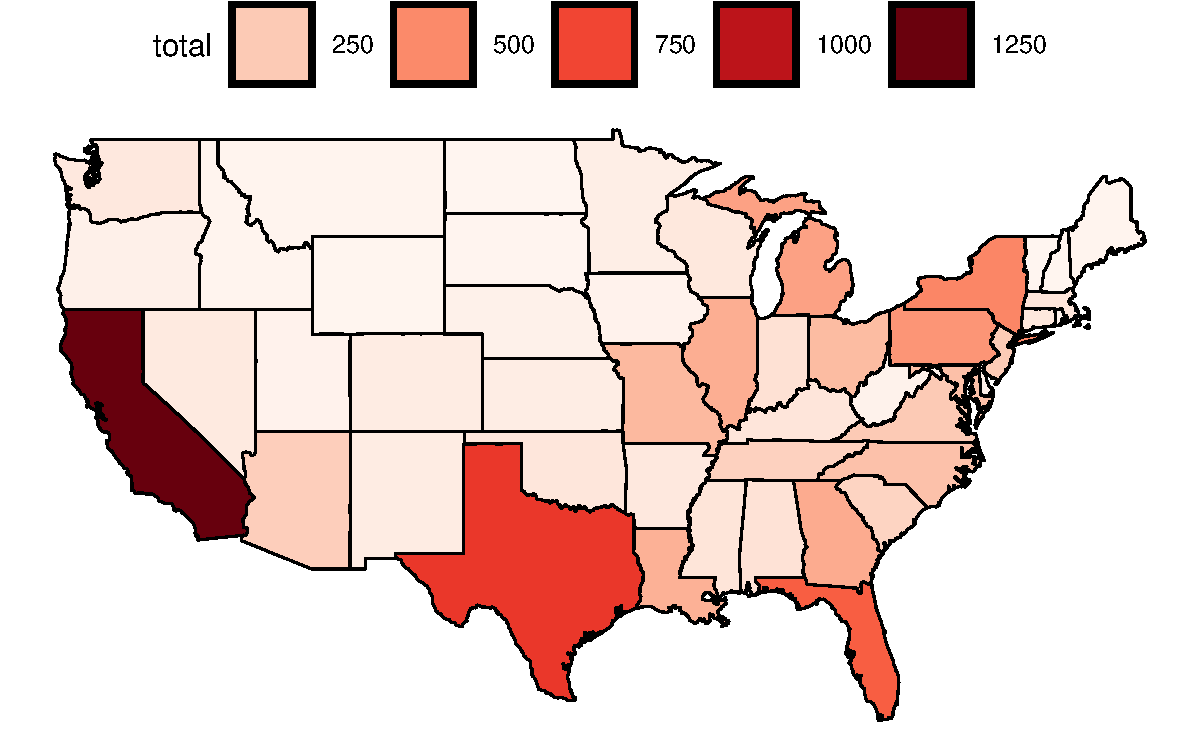
\includegraphics[width=0.99\linewidth]{PlotsLec4/UsaMapMurderPlt}
\end{figure}
\end{frame}

\end{document} 